% How to draw bar chart using tikz?
% https://tex.stackexchange.com/questions/99832/how-to-draw-bar-chart-using-tikz

\documentclass[border=5mm] {standalone}
\usepackage{pgfplots, pgfplotstable}


\begin{document}

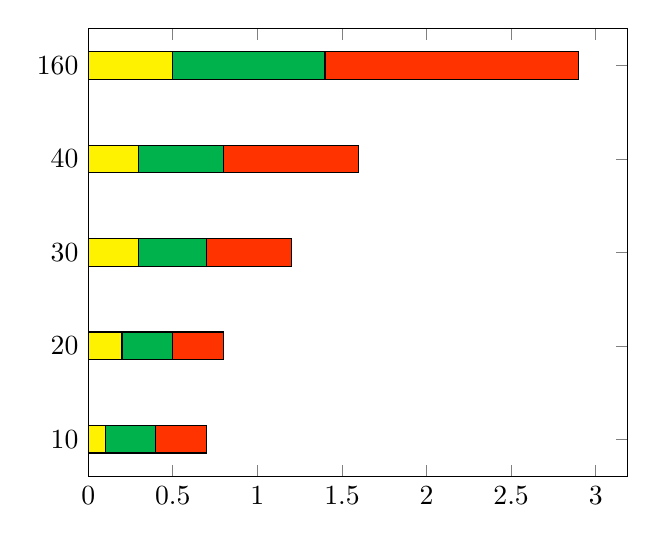
\begin{tikzpicture}
\pgfplotstableread{ % Read the data into a table macro
Label   First   Second  Third
10      0.1     0.3     0.3
20      0.2     0.3     0.3
30      0.3     0.4     0.5
40      0.3     0.5     0.8
160     0.5     0.9     1.5
}\datatable

\begin{axis}[
    xbar stacked,   % Stacked horizontal bars
    xmin=0,         % Start x axis at 0
    ytick=data,     % Use as many tick labels as y coordinates
    yticklabels from table={\datatable}{Label}  % Get the labels from the Label column of the \datatable
]
\addplot [fill=yellow] table [x=First, y expr=\coordindex] {\datatable};    % Plot the "First" column against the data index
\addplot [fill=green!70!blue]table [x=Second, y expr=\coordindex] {\datatable};
\addplot [fill=red!80!yellow] table [x=Third, y expr=\coordindex] {\datatable};
\end{axis}
\end{tikzpicture}

\end{document}
